\documentclass[onecolumn, draftclsnofoot,10pt, compsoc]{IEEEtran}
\usepackage{graphicx}
\usepackage{url}
\usepackage{setspace}
\usepackage{enumitem}
\usepackage{geometry}
\usepackage{pgfgantt}
\usepackage{float}
\usepackage{caption}
\captionsetup{justification=centering}

\geometry{textheight=9.5in, textwidth=7in}

\usepackage[parfill]{parskip}

\usepackage{fancyvrb}
\usepackage{color}
\usepackage[latin1]{inputenc}


\makeatletter
\def\PY@reset{\let\PY@it=\relax \let\PY@bf=\relax%
    \let\PY@ul=\relax \let\PY@tc=\relax%
    \let\PY@bc=\relax \let\PY@ff=\relax}
\def\PY@tok#1{\csname PY@tok@#1\endcsname}
\def\PY@toks#1+{\ifx\relax#1\empty\else%
    \PY@tok{#1}\expandafter\PY@toks\fi}
\def\PY@do#1{\PY@bc{\PY@tc{\PY@ul{%
    \PY@it{\PY@bf{\PY@ff{#1}}}}}}}
\def\PY#1#2{\PY@reset\PY@toks#1+\relax+\PY@do{#2}}

\expandafter\def\csname PY@tok@gd\endcsname{\def\PY@tc##1{\textcolor[rgb]{0.63,0.00,0.00}{##1}}}
\expandafter\def\csname PY@tok@gu\endcsname{\let\PY@bf=\textbf\def\PY@tc##1{\textcolor[rgb]{0.50,0.00,0.50}{##1}}}
\expandafter\def\csname PY@tok@gt\endcsname{\def\PY@tc##1{\textcolor[rgb]{0.00,0.25,0.82}{##1}}}
\expandafter\def\csname PY@tok@gs\endcsname{\let\PY@bf=\textbf}
\expandafter\def\csname PY@tok@gr\endcsname{\def\PY@tc##1{\textcolor[rgb]{1.00,0.00,0.00}{##1}}}
\expandafter\def\csname PY@tok@cm\endcsname{\let\PY@it=\textit\def\PY@tc##1{\textcolor[rgb]{0.25,0.50,0.50}{##1}}}
\expandafter\def\csname PY@tok@vg\endcsname{\def\PY@tc##1{\textcolor[rgb]{0.10,0.09,0.49}{##1}}}
\expandafter\def\csname PY@tok@m\endcsname{\def\PY@tc##1{\textcolor[rgb]{0.40,0.40,0.40}{##1}}}
\expandafter\def\csname PY@tok@mh\endcsname{\def\PY@tc##1{\textcolor[rgb]{0.40,0.40,0.40}{##1}}}
\expandafter\def\csname PY@tok@go\endcsname{\def\PY@tc##1{\textcolor[rgb]{0.50,0.50,0.50}{##1}}}
\expandafter\def\csname PY@tok@ge\endcsname{\let\PY@it=\textit}
\expandafter\def\csname PY@tok@vc\endcsname{\def\PY@tc##1{\textcolor[rgb]{0.10,0.09,0.49}{##1}}}
\expandafter\def\csname PY@tok@il\endcsname{\def\PY@tc##1{\textcolor[rgb]{0.40,0.40,0.40}{##1}}}
\expandafter\def\csname PY@tok@cs\endcsname{\let\PY@it=\textit\def\PY@tc##1{\textcolor[rgb]{0.25,0.50,0.50}{##1}}}
\expandafter\def\csname PY@tok@cp\endcsname{\def\PY@tc##1{\textcolor[rgb]{0.74,0.48,0.00}{##1}}}
\expandafter\def\csname PY@tok@gi\endcsname{\def\PY@tc##1{\textcolor[rgb]{0.00,0.63,0.00}{##1}}}
\expandafter\def\csname PY@tok@gh\endcsname{\let\PY@bf=\textbf\def\PY@tc##1{\textcolor[rgb]{0.00,0.00,0.50}{##1}}}
\expandafter\def\csname PY@tok@ni\endcsname{\let\PY@bf=\textbf\def\PY@tc##1{\textcolor[rgb]{0.60,0.60,0.60}{##1}}}
\expandafter\def\csname PY@tok@nl\endcsname{\def\PY@tc##1{\textcolor[rgb]{0.63,0.63,0.00}{##1}}}
\expandafter\def\csname PY@tok@nn\endcsname{\let\PY@bf=\textbf\def\PY@tc##1{\textcolor[rgb]{0.00,0.00,1.00}{##1}}}
\expandafter\def\csname PY@tok@no\endcsname{\def\PY@tc##1{\textcolor[rgb]{0.53,0.00,0.00}{##1}}}
\expandafter\def\csname PY@tok@na\endcsname{\def\PY@tc##1{\textcolor[rgb]{0.49,0.56,0.16}{##1}}}
\expandafter\def\csname PY@tok@nb\endcsname{\def\PY@tc##1{\textcolor[rgb]{0.00,0.50,0.00}{##1}}}
\expandafter\def\csname PY@tok@nc\endcsname{\let\PY@bf=\textbf\def\PY@tc##1{\textcolor[rgb]{0.00,0.00,1.00}{##1}}}
\expandafter\def\csname PY@tok@nd\endcsname{\def\PY@tc##1{\textcolor[rgb]{0.67,0.13,1.00}{##1}}}
\expandafter\def\csname PY@tok@ne\endcsname{\let\PY@bf=\textbf\def\PY@tc##1{\textcolor[rgb]{0.82,0.25,0.23}{##1}}}
\expandafter\def\csname PY@tok@nf\endcsname{\def\PY@tc##1{\textcolor[rgb]{0.00,0.00,1.00}{##1}}}
\expandafter\def\csname PY@tok@si\endcsname{\let\PY@bf=\textbf\def\PY@tc##1{\textcolor[rgb]{0.73,0.40,0.53}{##1}}}
\expandafter\def\csname PY@tok@s2\endcsname{\def\PY@tc##1{\textcolor[rgb]{0.73,0.13,0.13}{##1}}}
\expandafter\def\csname PY@tok@vi\endcsname{\def\PY@tc##1{\textcolor[rgb]{0.10,0.09,0.49}{##1}}}
\expandafter\def\csname PY@tok@nt\endcsname{\let\PY@bf=\textbf\def\PY@tc##1{\textcolor[rgb]{0.00,0.50,0.00}{##1}}}
\expandafter\def\csname PY@tok@nv\endcsname{\def\PY@tc##1{\textcolor[rgb]{0.10,0.09,0.49}{##1}}}
\expandafter\def\csname PY@tok@s1\endcsname{\def\PY@tc##1{\textcolor[rgb]{0.73,0.13,0.13}{##1}}}
\expandafter\def\csname PY@tok@sh\endcsname{\def\PY@tc##1{\textcolor[rgb]{0.73,0.13,0.13}{##1}}}
\expandafter\def\csname PY@tok@sc\endcsname{\def\PY@tc##1{\textcolor[rgb]{0.73,0.13,0.13}{##1}}}
\expandafter\def\csname PY@tok@sx\endcsname{\def\PY@tc##1{\textcolor[rgb]{0.00,0.50,0.00}{##1}}}
\expandafter\def\csname PY@tok@bp\endcsname{\def\PY@tc##1{\textcolor[rgb]{0.00,0.50,0.00}{##1}}}
\expandafter\def\csname PY@tok@c1\endcsname{\let\PY@it=\textit\def\PY@tc##1{\textcolor[rgb]{0.25,0.50,0.50}{##1}}}
\expandafter\def\csname PY@tok@kc\endcsname{\let\PY@bf=\textbf\def\PY@tc##1{\textcolor[rgb]{0.00,0.50,0.00}{##1}}}
\expandafter\def\csname PY@tok@c\endcsname{\let\PY@it=\textit\def\PY@tc##1{\textcolor[rgb]{0.25,0.50,0.50}{##1}}}
\expandafter\def\csname PY@tok@mf\endcsname{\def\PY@tc##1{\textcolor[rgb]{0.40,0.40,0.40}{##1}}}
\expandafter\def\csname PY@tok@err\endcsname{\def\PY@bc##1{\setlength{\fboxsep}{0pt}\fcolorbox[rgb]{1.00,0.00,0.00}{1,1,1}{\strut ##1}}}
\expandafter\def\csname PY@tok@kd\endcsname{\let\PY@bf=\textbf\def\PY@tc##1{\textcolor[rgb]{0.00,0.50,0.00}{##1}}}
\expandafter\def\csname PY@tok@ss\endcsname{\def\PY@tc##1{\textcolor[rgb]{0.10,0.09,0.49}{##1}}}
\expandafter\def\csname PY@tok@sr\endcsname{\def\PY@tc##1{\textcolor[rgb]{0.73,0.40,0.53}{##1}}}
\expandafter\def\csname PY@tok@mo\endcsname{\def\PY@tc##1{\textcolor[rgb]{0.40,0.40,0.40}{##1}}}
\expandafter\def\csname PY@tok@kn\endcsname{\let\PY@bf=\textbf\def\PY@tc##1{\textcolor[rgb]{0.00,0.50,0.00}{##1}}}
\expandafter\def\csname PY@tok@mi\endcsname{\def\PY@tc##1{\textcolor[rgb]{0.40,0.40,0.40}{##1}}}
\expandafter\def\csname PY@tok@gp\endcsname{\let\PY@bf=\textbf\def\PY@tc##1{\textcolor[rgb]{0.00,0.00,0.50}{##1}}}
\expandafter\def\csname PY@tok@o\endcsname{\def\PY@tc##1{\textcolor[rgb]{0.40,0.40,0.40}{##1}}}
\expandafter\def\csname PY@tok@kr\endcsname{\let\PY@bf=\textbf\def\PY@tc##1{\textcolor[rgb]{0.00,0.50,0.00}{##1}}}
\expandafter\def\csname PY@tok@s\endcsname{\def\PY@tc##1{\textcolor[rgb]{0.73,0.13,0.13}{##1}}}
\expandafter\def\csname PY@tok@kp\endcsname{\def\PY@tc##1{\textcolor[rgb]{0.00,0.50,0.00}{##1}}}
\expandafter\def\csname PY@tok@w\endcsname{\def\PY@tc##1{\textcolor[rgb]{0.73,0.73,0.73}{##1}}}
\expandafter\def\csname PY@tok@kt\endcsname{\def\PY@tc##1{\textcolor[rgb]{0.69,0.00,0.25}{##1}}}
\expandafter\def\csname PY@tok@ow\endcsname{\let\PY@bf=\textbf\def\PY@tc##1{\textcolor[rgb]{0.67,0.13,1.00}{##1}}}
\expandafter\def\csname PY@tok@sb\endcsname{\def\PY@tc##1{\textcolor[rgb]{0.73,0.13,0.13}{##1}}}
\expandafter\def\csname PY@tok@k\endcsname{\let\PY@bf=\textbf\def\PY@tc##1{\textcolor[rgb]{0.00,0.50,0.00}{##1}}}
\expandafter\def\csname PY@tok@se\endcsname{\let\PY@bf=\textbf\def\PY@tc##1{\textcolor[rgb]{0.73,0.40,0.13}{##1}}}
\expandafter\def\csname PY@tok@sd\endcsname{\let\PY@it=\textit\def\PY@tc##1{\textcolor[rgb]{0.73,0.13,0.13}{##1}}}

\def\PYZbs{\char`\\}
\def\PYZus{\char`\_}
\def\PYZob{\char`\{}
\def\PYZcb{\char`\}}
\def\PYZca{\char`\^}
\def\PYZam{\char`\&}
\def\PYZlt{\char`\<}
\def\PYZgt{\char`\>}
\def\PYZsh{\char`\#}
\def\PYZpc{\char`\%}
\def\PYZdl{\char`\$}
\def\PYZti{\char`\~}
% for compatibility with earlier versions
\def\PYZat{@}
\def\PYZlb{[}
\def\PYZrb{]}
\makeatother


\newcommand{\subparagraph}{}

% Reformat section and subsection styles
\usepackage{titlesec}
\setcounter{secnumdepth}{4}

\titleformat{\section}
{\normalfont\huge\bfseries\sffamily}{\thesection}{1em}{}

\titleformat{\subsection}
{\normalfont\large\bfseries\sffamily}{\thesubsection}{1em}{}

\titleformat{\subsubsection}
{\normalfont\normalsize\bfseries\sffamily}{\thesubsubsection}{1em}{}

\titleformat{\paragraph}
{\normalfont\normalsize\sffamily\itshape}{\theparagraph}{2em}{}


% 1. Fill in these details
\def \CapstoneTeamName{     }
\def \CapstoneTeamNumber{       36}
\def \GroupMemberOne{           Trevor Swope}
\def \GroupMemberTwo{           William Selbie}
\def \GroupMemberThree{         Luke Goertzen}
\def \CapstoneProjectName{      Project LOOM}
\def \CapstoneSponsorCompany{   Openly Published Environmental Sensing Lab}
\def \CapstoneSponsorPerson{    Chet Udell}

% 2. Uncomment the appropriate line below so that the document type works
\def \DocType{  %Problem Statement
                %Requirements Document
                % Technology Review
                Preliminary Design Document
                %Progress Report
                }
            
\newcommand{\NameSigPair}[1]{\par
\makebox[2.75in][r]{#1} \hfil   \makebox[3.25in]{\makebox[2.25in]{\hrulefill} \hfill        \makebox[.75in]{\hrulefill}}
\par\vspace{-12pt} \textit{\tiny\noindent
\makebox[2.75in]{} \hfil        \makebox[3.25in]{\makebox[2.25in][r]{Signature} \hfill  \makebox[.75in][r]{Date}}}}
% 3. If the document is not to be signed, uncomment the RENEWcommand below
%\renewcommand{\NameSigPair}[1]{#1}

%%%%%%%%%%%%%%%%%%%%%%%%%%%%%%%%%%%%%%%
\begin{document}
\begin{titlepage}
    \pagenumbering{gobble}
    \begin{singlespace}
        % \includegraphics[height=4cm]{coe_v_spot1}
        \hfill 
        % 4. If you have a logo, use this includegraphics command to put it on the coversheet.
        %\includegraphics[height=4cm]{CompanyLogo}   
        \par\vspace{.2in}
        \centering
        \scshape{
            \huge CS Capstone \DocType \par
            {\large\today}\par
            \vspace{.5in}
            \textbf{\Huge\CapstoneProjectName}\par
            \vfill
            {\large Prepared for}\par
            \Huge Kevin McGrath \\ Kirsten Winters \par
            \vspace{5pt}
            % {\Large\NameSigPair{\CapstoneSponsorPerson}\par}
            {\large Prepared by }\par
            Group\CapstoneTeamNumber\par
            % 5. comment out the line below this one if you do not wish to name your team
            \CapstoneTeamName\par 
            \vspace{5pt}
            % {\Large
            %     \NameSigPair{\GroupMemberOne}\par
            %     \NameSigPair{\GroupMemberTwo}\par
            %     \NameSigPair{\GroupMemberThree}\par
            % }
            \GroupMemberOne \\
            \GroupMemberTwo \\
            \GroupMemberThree \\
            \vspace{20pt}
        }
        \begin{abstract}
            This document presents the design decisions, elements, justifications, and processes of building and implementing the core components of Group 36's portion of Project LOOM.
        \end{abstract}     
    \end{singlespace}
\end{titlepage}
\newpage
\pagenumbering{arabic}
\tableofcontents
% 7. uncomment this (if applicable). Consider adding a page break.
% \listoffigures
% \listoftables
\clearpage

\section{Introduction}
\subsection{Scope}  
    With Project LOOM, we aim to create an open-source, plug-and-play, suite of modular building blocks, the extensible and easy programmability of which expands the demographic of people capable of implementing Internet of Things solutions. For users with limited technical expertise to create complex systems, we aim to build a system that abstracts out the more technical details, allowing them to focus on their system more than the implementation of the modules. The system should also be usable by higher level students and experts by allowing them to modify or write their own firmware, and create new modules. Project LOOM will be developed for university faculty demos of functionality. Possible subsequent commercialization is currently outside of the scope of the Senior Capstone project.

\subsection{Purpose}
    This design document is intended to be used as a map of the planned design decisions and process for Group 36's portion of the implementation of Project LOOM as described in the scope section above.
                
\subsection{Intended audience}
    This document is intended for use by Capstone Group 36, the Capstone instructors, and the Project LOOM client as the official documentation of design decisions for the main components of the project. The rationale behind each decision is provided, as is the method of implementation.

\subsection{Reference Material}
    \renewcommand{\listfigurename}{}
    \vspace{-40pt}
    \listoffigures

\section{Glossary}
    \textbf{Gateway:} A wired or wireless node connecting multiple devices on a network (e.g. via WiFi or Ethernet)

    \textbf{Internet of Things (IoT) Network:} Entails an aggregate of systems (many of which are embedded) capable of reading, transmitting, receiving, processing, and acting upon data. This often takes the form of a network of remotely connected devices that can be used for the purpose of autonomous data collection, or remote control and automation of various systems.

    \textbf{I/O:} input and output

    \textbf{LOOM Kit:} A set of pre-assembled modules with specific input and output capabilities that will be produced and distributed as an end goal of Project LOOM. Each kit should have the potential to be its own IoT Network. 

    \textbf{Module:} An interchangeable, self-contained device that can be connected to an IoT network with minimal configuration. Connects to other modules to combine behaviors (e.g. a sensor attached to a WiFi adapter becomes a sensor that transfers data over WiFi).

    \textbf{Shield:} A circuit board that can be attached to another processor to extend the latter's functionality. The combination of microprocessors and shields will be used to make modules.




\section{Design Interests and Views}
\subsection{Design Stakeholders and Interests}

\subsubsection{Project LOOM Client}
    Dr. Chet Udell

    Interests: Wants a functional, modular Internet of Things Rapid Prototyping System, and proofs of concept to demonstrate it.

\subsubsection{Other Project LOOM Developers}
    Designers contributing to Project LOOM that are not part of the Group 36 developer subset

    Interests: Will need to be able to work with and around any design decisions or systems made by Group 36.

\subsubsection{Users}
    The eventual users of the Project LOOM Rapid Internet of Things Prototyping System

    Interests: Should be able to easily use the system designed and implemented by Project LOOM developers.

\subsection{Design Views}
    There are a variety of perspectives that stakeholders might hold when viewing Project LOOM. In order of decreasing abstraction they are:

\subsubsection{User View}
    As Project LOOM is being developed for users, the users are going to see the system in a different way than the developers. They are going to be concerned with the user interfaces and what the IoT modules do, not necessarily how they do so. This view is one of the highest level views, as most users will not need to be presented with the implementation details.

\subsubsection{Developer View}
    The Project LOOM developers need to be able to see the interactions of the modules that are being produced and programmed. They do not always necessarily need to know how another developer implemented a module's functionality, but they should be able to get an overview of the entire system, and the relationships and interactions between components.

\subsubsection{Communication View}
    The communication between components of an Internet of Things system is important, but is generally best left abstracted out of most views. Some developers only need to know that modules are communicating, perhaps distinguishing between wired and wireless, not needing the details of which protocol or format is in use. These details are described in the Communication View.





\section{Design}
\subsection{User Viewpoint: Context}
    The users of the Project LOOM rapid Internet of Things prototyping system are going to need to be able to interact with their project. They should also have the option to connect a variety of other software and services to their hardware setups. There are three primary aspects of the user experience that can be examined while abstracting most of the underlying functionality into a "black box" to be discussed in other viewpoints. These three are as follows: the user interface; external visualization of I/O; and events and notifications.

\subsubsection{User Interface}
    The purpose of the user interface of Project LOOM is to provide the users with a graphical interface that allows them to visually design, setup, monitor, and control their Internet of Things project. The user interface should incorporate different ways of displaying the states of the connected modules and the streams of data to and from said modules. Modifications to or calibration of the network of devices should also be permitted through the user interface.

\paragraph{Authorship}
    Luke Goertzen

\paragraph{Design Concerns}
    As Project LOOM is directed at a diverse audience, ranging from K-12 to college students and professional users, the associated user interface needs to be able to serve a variety of groups without being either intimidating or restricting. The software should be easy to understand and use by beginners to the IoT field while still providing more experienced users the flexibility to customize and write their own code for the software. Additionally, the user interface should be able to run on multiple operating systems for the user's convenience.

    The user interface should easily connect to the IoT modules developed in the rest of Project LOOM and be able to clearly display information about an IoT setup of those modules. It is also important that the software be reasonably priced, so that the varied audience can afford to build an Internet of Things network with Project LOOM modules and interface.

    Summary of Criteria:
    \begin{itemize}[noitemsep,topsep=-10pt]
        \item Easy to use
        \item Advanced features available
        \item Extensible by users
        \item Multiple operating system support
        \item Low cost
    \end{itemize}

\paragraph{Design Elements}
    Max/MSP will be used to implement the user interface. Max/MSP is a modular, visual programming interface developed by Cycling '74 primarily for use in controlling interactive music and multimedia. The software can be enhanced with extended functionality through creating new objects via a provided API or by writing code in Java or Javascript. Additionally, the user interface one designs with Max for their project is not entirely distinct from the program structure itself. The functionality of the program is primarily developed graphically, and a presentation mode allows the user to modify the layout and appearance of the program objects to create an interface, without affecting the underlying program flow. Max can easily be connected to microprocessors such as Arduino, and receive input from and output to a variety peripherals, including controllers, DMX lighting, projectors, and audio. \cite{max}

    The full version of Max costs \$399, or about \$8-10 per month for a subscription depending on the subscription length, with discounts available for students. The software runs on both Windows and macOS, and can be connected to an iPad via Cycling '74's Mira app. \cite{buymax}

\paragraph{Design Rationale}
    Max/MSP was selected to fill this role as the base of the user interface because it is relatively affordable compared to similar programs such as LabVIEW, while also running on more operating systems. LabVIEW is a professional testing tool, but is not well suited to build an interface off of. Max, on the other hand, is intended to be used with existing software and hardware. In addition, Max's close relation between the program - the coordination of input and output, and processing - and the interface accomplishes two tasks at once and would likely be appreciated by less experienced users.

\paragraph{Design Implementation}
    The user interface will be designed as processing modules. These modules contain a set of similar functions and can receive and output streams of data. Modules can be linked together to pass information from one to another. The Project LOOM client, Dr. Chet Udell, has prepared a base set of data processor modules that can be used in Max. The set of data processor plugins provided by Dr. Udell include different ways of reading information from a network, a variety of modules to process, convert, or display this information, and modules to send data back out to the network. As more hardware or specialized needs arise, more modules can be developed to provide relevant displays, processing, and I/O. The modules encapsulate objects and program, but can be opened and modified by both developers and users to tailor their (the modules') functionality.

    \begin{figure}[H]
        \centering
        \caption{NeoPixel Presentation View}
        \label{fig:neopixel_pres}
        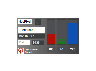
\includegraphics[width=8cm]{neopixel_presentation.eps}         
     \end{figure}

     \begin{figure}[H]
        \centering
        \caption{Edit NeoPixel Module}
        \label{fig:neopixel_edit}
        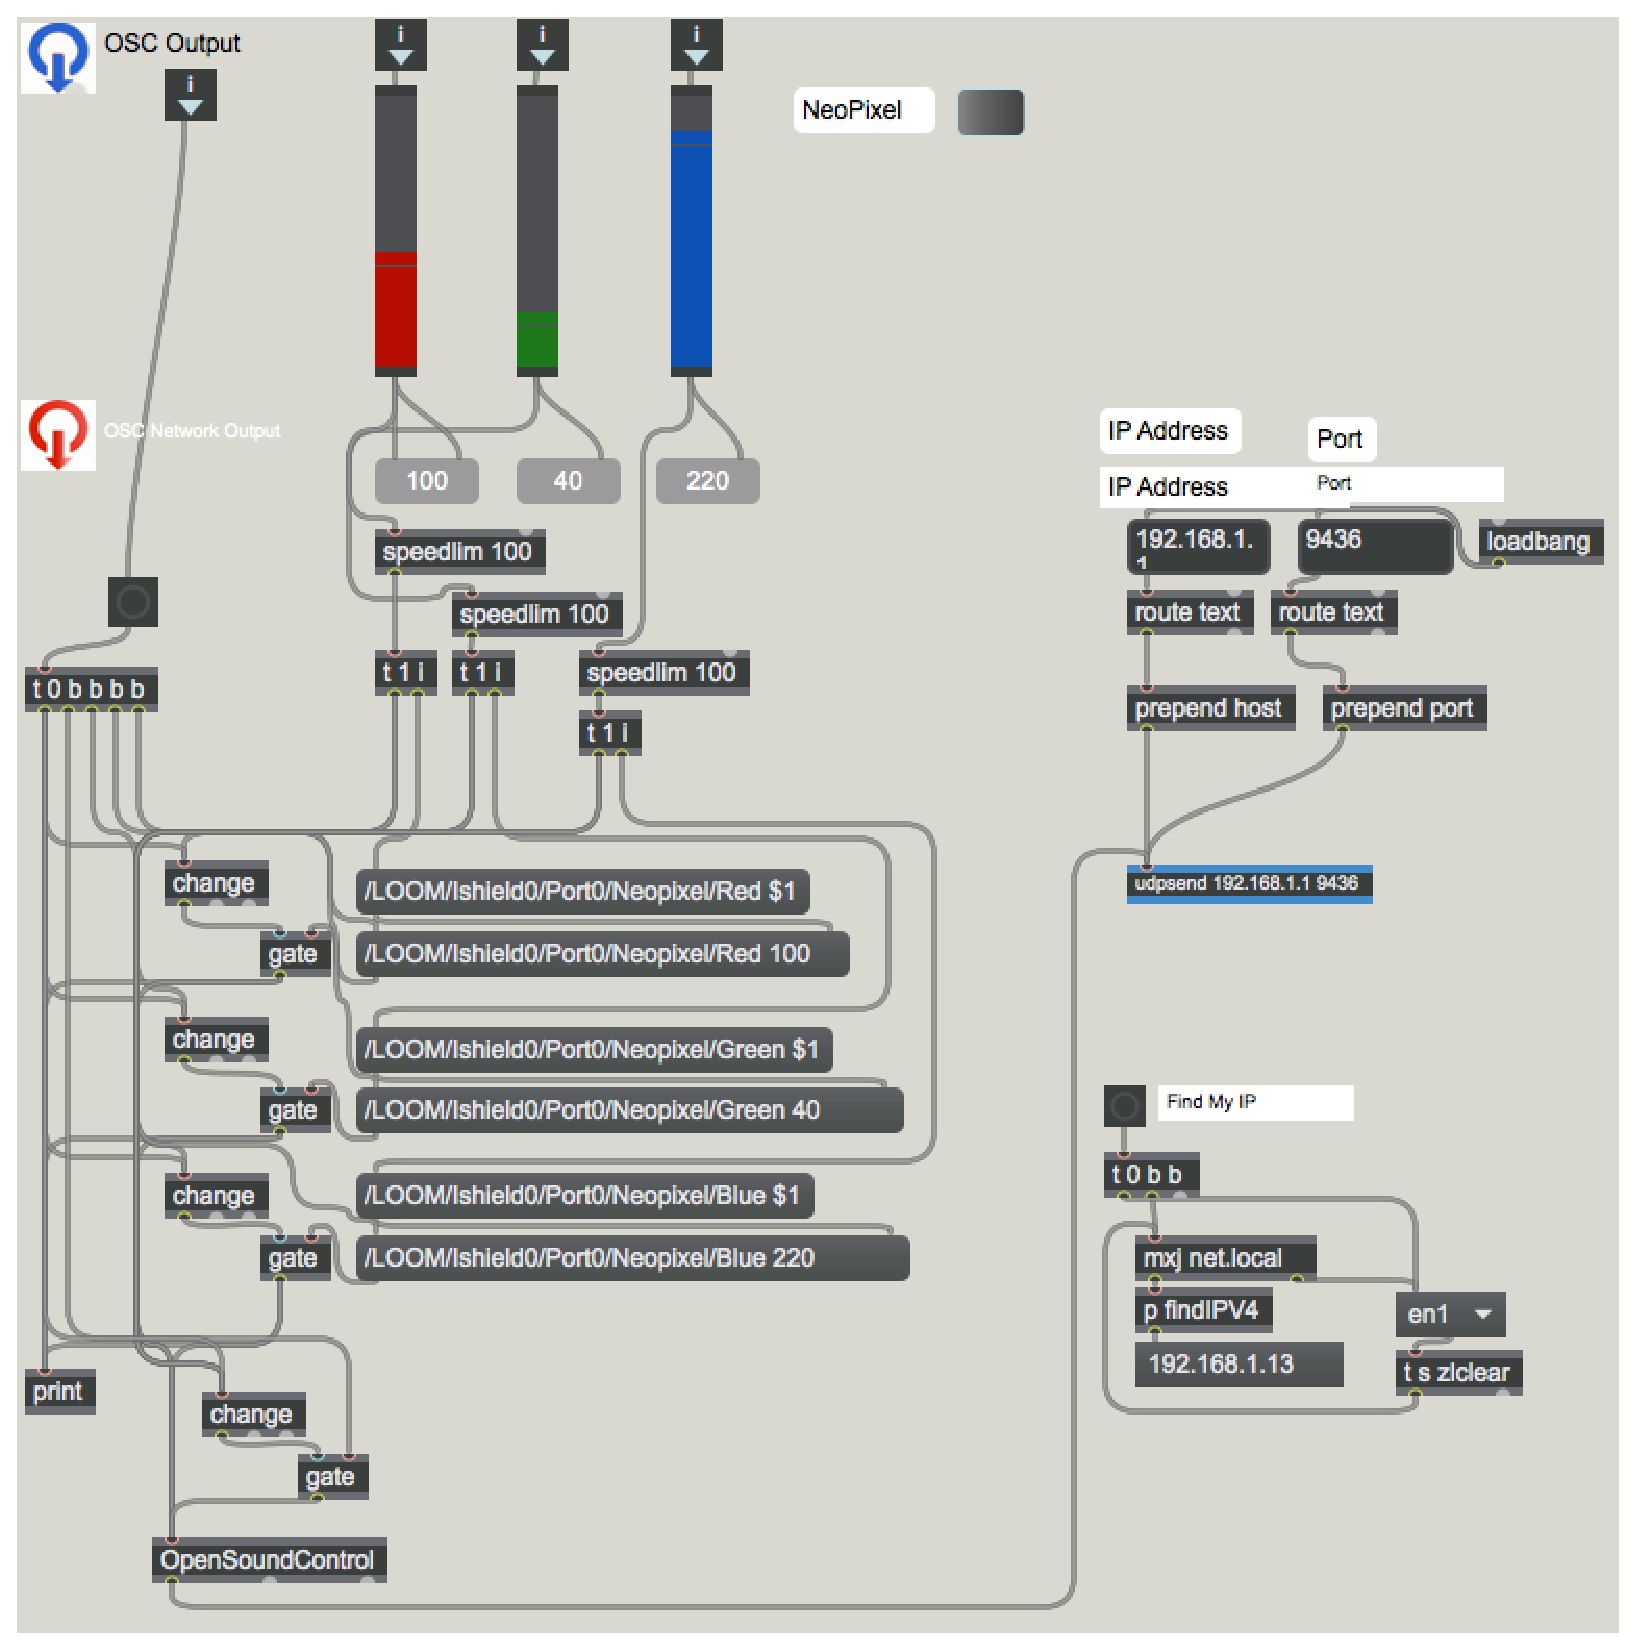
\includegraphics[width=10cm]{neopixel_edit.eps}         
     \end{figure}


\subsubsection{External Visualization of I/O}
    A core purpose of an Internet of Things network is to gather and act upon data. Users should be able to easily view and interpret the readings and state of their network. In addition to the user interface for configuring an Internet of Things system and subsequently monitoring and directing its I/O, Project LOOM aims to provide users with a multiple ways of outputting data from the network. While the user interface will feature some display capabilities, linking separate display systems and logging services can allow a user to find the best setup for their needs. As such, Project LOOM aims to support interfacing with a variety of external services, as opposed to limiting itself to one.

\paragraph{Authorship}
    Luke Goertzen

\paragraph{Design Concerns}
    The external visualization of I/O component of Project LOOM can be addressed with one of a variety of services, however, providing users with multiple supported options reduces the probability that design decisions made by the developers are restrictive to the users. Further, an approximate priority will be presented as to the order in which solutions will planned for implementation.

    Each feasible visualization option will need to easily connect to an IoT network (from the user's perspective) and user be able to use the variety of services it may present. There is preference to the options that are cheaper, if not free, as that expands the audience that can fully use Project LOOM.

    Summary of Criteria:
    \begin{itemize}[noitemsep,topsep=-10pt]
        \item Easy connection to IoT network
        \item Easy to use and understand
        \item Variety of services
        \item Low cost is preferable
    \end{itemize}

\paragraph{Design Elements}
    Project LOOM plans to interface with both Adafruit IO and Plotly to provide visualization of data extracted from an Internet of Things network.

    Adafruit produces a variety of hardware devices, including a number that are intended specifically for Internet of Things projects - some of which already in use by Project LOOM. The company (Adafruit) made Adafruit IO to better drive and monitor IoT setups constructed from both their own devices and third-party devices. Adafruit IO is well documented and has an established community of makers. Adafruit IO has two pricing tiers for users, a perpetual free version and a \$10 full version.

    Adafruit IO provides an API to easily let users interact with I/O from a variety of interfaces and prepare dashboards based off of data feeds for powerful displays. \cite{adafruitio}

    Plotly is similar to Adafruit IO in that it provides dashboards and visualizations of data. Plotly is a professional tool used by large companies in industry and provides options for advanced graphical outputs of the data supplied. This data can be read straight from a database, or can be imported from common formats such as Excel or CSV. Plotly can be used to create graphs and charts with provided APIs and open source libraries of Python, R, MATLAB, and JavaScript (including the powerful visualization library D3.js). Pricing for Plotly ranges from free to professional tiers. \cite{plotly}

\paragraph{Design Rationale}
    Adafruit IO allows for control and interactions with the IoT devices in a network. Additionally, the large community and extensive documentation of Adafruit IO are likely beneficial for the beginner-level users of Project LOOM, and can be convenient for the developers as well.

    Plotly is not specifically directed at IoT applications and does not provide interaction with the network of devices. However, it can be used for generating graphics based on the data said network collects, and is capable of creating more elaborate and interactive visualizations than Adafruit IO can.

\paragraph{Design Implementation}
    The external visualizations of Project LOOM networks will be handled by the connected platforms, Adafruit IO and Plotly. The role of the developers is to get the information out of the network and to these services. This can be done continuously, in which data would sent to the service at regular intervals, or all at once, in which a set of data is collected and then sent processed all at once. 

    Communication with the two services is simple, entailing the usage of the provided APIs and/or formatting files correctly (e.g. CSV file).

    Users and developers can then use the tools' provided functionalities to design logs, dashboards, charts, and graphs. At this stage, design decisions are generally no longer those of Project LOOM, but of the companies providing the services. Users still will have the freedom to design their visualizations as they please.


\subsubsection{Events and Notifications}
    The solutions in this section are intended to allow users to incorporate pre-existing (non-Project LOOM) devices, software, and services into a LOOM network. This includes using user input as triggers to the network and having the network output information to a variety of locations and services beyond the configuration user interface and data visualization. Notifications can keep a user informed about important occurrences with the network. The user should also be able to automate output actions of the network.

\paragraph{Authorship}
    Luke Goertzen

\paragraph{Design Concerns}
    Project LOOM intends to interface with multiple services that provide events and/or notifications from a network of devices to suit the varied needs of users. The services should be easy for users to incorporate into an IoT network and use. Although each option may not feature both events and notifications, between all supported options there should be the potential for user input and automated network output. Low cost is preferred if possible.

    Summary of Criteria:
    \begin{itemize}[noitemsep,topsep=-10pt]
        \item Easy to use and add to network
        \item Allows user input to network
        \item Automation of events
        \item Notifications
        \item Low cost
    \end{itemize}

\paragraph{Design Elements}
    Project LOOM plans to interface with Adafruit IO, IFTTT and PushingBox (if necessary) to handle events and notifications to and from an IoT network.

    Adafruit IO, which is planned for use in the External Visualization of I/O component of Project LOOM, also has applications for events and notifications. For example, a user can set up a trigger to watch for certain events or changes in the network, responding with an output such as a notification to the user. Alternatively, using Adafruit IO can allow the network to get data from or send data to a web browser. \cite{adafruitio}

    IFTTT is a popular, free platform for establishing interactions between many different consumer applications and devices. The service runs via the web and a suite of apps for iOS and Android. IFTTT stands for IF This Then That, and is used to build recipes of conditions and corresponding actions should those conditions be met. Meaning that if X happens by some event or user action, then event Y should be triggered. This allows for the automation of common sequences of actions that a user may perform or check for. \cite{ifttt}

    PushingBox provides a simple API for triggering actions via HTTP requests or emails and directed to a variety of services. These triggers can come from many sources, including Arduino (or other microprocessors), the aforementioned IFTTT, and custom scripts. PushingBox currently supports actions such as notifications to many operating systems, emails, HTTP requests, or writing to Google Docs. Usage of the PushingBox API is free. \cite{pushingbox}

\paragraph{Design Rationale}
    While some of the listed systems above have overlapping features, support for all of them permits users the widest variety of options. All can be used for free, however, among the three, IFTTT is the most refined, while PushingBox is the least. As such, IFTTT has more options for triggers and actions than PushingBox does, possibly making the latter redundant to support. Further, IFTTT is more user-friendly to use. Adafruit falls somewhere in between compared to the other two, but has the other uses as presented in the External Visualization of I/O. If the user is already using Adafruit for monitoring, it would not be much more effort to include triggers and events. Again, Adafruit's documentation, community, and examples make the platform enticing for users.

    Based on the refinement and features, Adafruit and IFTTT will likely be prioritized for support. It may also be possible to use IFTTT to do everything that PushingBox does, thus eliminating the need for the latter. This will be determined as these begin being implemented. Regardless of which ones are implemented, they are generally all able to work with the others.

\paragraph{Design Implementation}
    The events and notifications component of Project LOOM exists to extend the network to include applications and services not developed by LOOM. As such, the main goal of the developers here is to simply interface with the external components, giving access to data streams for the components to act upon or react to. The components will either: pass the data from one section of the network to another, examine the data for conditions to trigger events, or send data from the user into the network.

    Interfacing with these components will primarily entail using the associated APIs to send or receive information. Project LOOM will design sample interactions with these services to demonstrate how they could be used.






\subsection{Developer Viewpoint: Composition}
    This viewpoint is primarily applicable to the Project LOOM developers, as to be able to see the relationships between all modules, devices, and software of the system. The composition of the project will depict these relationships, along with the overall architecture that describes the nature and structure of the relationships between the modules and gateways in an IoT network.

\subsubsection{Network Architecture}
    The architecture of the network will determine the route that data will take from its starting point (the source of the input or data), to its ending point (wherever the data is sent to last). This route starts with either the modules attached to sensors or user input, but after that point then the route taken is entirely architecture dependent. 

    The ideal network architecture is:
    \begin{itemize}[noitemsep,topsep=-10pt]
        \item Simple to implement
        \item Flexible in how it can be applied,
        \item Extensible in its ability to be scaled up or down in size. 
    \end{itemize}

\paragraph{Authorship}
    Project LOOM Developers

\paragraph{Design Concerns}
    Each IoT network will be capable of gathering certain inputs and giving certain outputs, which will be dependent upon the modules in the LOOM kit. In any given LOOM kit, each module is going to be capable of at least two of the following functions:

    \begin{itemize}[noitemsep,topsep=-10pt]
        \item Gathering data from a sensor
        \item Performing an action with an actuator
        \item Transmitting data to another device on the network
        \item Receiving data from another device on the network
        \item Processing gathered or received data
        \item Transmitting data to a device connected to the world wide web\\
    \end{itemize}
    
    However, not all of the modules will need to perform each of these functions, so it is necessary to decide how the network will be architected to make the most efficient use of the kits' resources. 

    The criteria upon which network structures will be evaluated are: 
    \begin{itemize}[noitemsep,topsep=-10pt]
        \item Cost efficiency of required modules
        \item Flexibility of application
        \item Extensibility
    \end{itemize}

\paragraph{Design Elements}
    Project LOOM plans to implement a Gateway Centralized architecture, wherein each node in the network is either a module or a gateway. Modules are capable of gathering and transmitting data, or actuating and receiving data. Modules gathering data will periodically transmit data to a the network's gateway. The gateway will process the data, and if certain criteria are met, send commands to the modules. The gateway can also transmit the received and processed data to some external system, such as the aforementioned Plotly and Adafruit IO. 

\paragraph{Design Rationale}
    Gateway centralization is a cost efficient and extensible architecture because of the specialization that it requires in each module. By minimizing the required functionality in each module while still maintaining the same overall system capabilities, each module will be cheaper and simpler to use with no overall loss in what the IoT network as a whole can achieve. It is also more extensible as the structure can be used recursively wherein the gateways in each of several smaller IoT networks can transmit aggregate data to the gateway of a larger network. With this method of usage, the architecture can be applied to networks and projects of any size.

\paragraph{Design Implementation}
    Project LOOM will implement a gateway centralized network by having each module in the network with the same wireless communication platform send data to and receive data from a central node, the gateway. The gateway would then be the only node in the network responsible for transmitting data to its end destination, regardless of where that is. Each module will be capable of wireless communication, which it will use to send packets of data to the gateway or receive packets from the gateway. The gateway will upon receiving packets then process them accordingly and send the processed packets of data to the next recipient, either in the IoT network or outside of it. 

    \begin{figure}[H]
        \centering
        \caption{Network Architecture}
        \label{fig:network_architecture}
        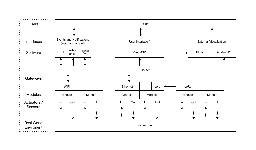
\includegraphics[width=16cm]{network_architecture.eps}         
     \end{figure}


\subsubsection{Module Control Structure}
    The module control structure will determine where the instructions and routines that the modules follow come from. The control structure could range from each module solely providing their own instructions, to modules containing no internal instructions. The ideal module control structure for Project LOOM is somewhere in between, such that modules can be autonomous enough to be simple and robust, but allows for enough external control to make the system flexible.

\paragraph{Authorship}
    William Selbie

\paragraph{Design Concerns}
    Each module in the IoT network will be capable of gathering data or using an actuator of some kind, and a crucial question that goes with this is, "How will the actions of each of the modules in the network be decided?". The answer being that the modules can be controlled in a variety of ways, each with benefits and drawbacks. The control structure will be chosen based on the following criteria:
    \begin{itemize}[noitemsep,topsep=-10pt]
        \item Firmware leanness
        \item Flexibility of application
        \item Extensibility
        \item Robustness
    \end{itemize}

\paragraph{Design Elements}
    Project LOOM plans to control each module mainly through use of the gateway, wherein each module would be programmed with all the routines needed to gather, transmit, and receive data. Each module could then potentially have initial startup and looping routines that would be run in at intervals set when the firmware was loaded onto the module. These modules would then be able to receive instructions from the gateway that could modify or replace the initial routines, or simply call a specific routine once. This would allow for the modules to have simple autonomy without forcing that paradigm onto the user. It also gives the user the ability to make use of any of the capabilities of any module at any time. This gives the user complete control and flexibility in how they would like to make use of their modules' capabilities.

\paragraph{Design Rationale}
    The gateway oriented module control structure maximizes the flexibility of the IoT network by allowing for both automated and manual access to each of the modules' capabilities. This does result in firmware that is less lean than the alternate control structures, but not so bloated as to be an impossible or unreasonable implementation. Beyond this the potential for simple autonomy of each of the modules means the system is robust when desired, as faulty input from the gateway wouldn't prevent succesful data gathering. The natural flexibility of how the modules can be controlled also lends to the extensibility of the IoT networks and kits as a whole. 

\paragraph{Design Implementation}
    Each Project LOOM module's firmware contains the same basic structure that includes a series of instructions to run once when the module is turned on, and then another series of instructions to continuously run in a loop while the device is on. In a gateway oriented module control structure, the module's instructions that it looped through would involve receiving and parsing instructions being sent to it by the gateway. Along with this, modules would also have the capability to have a set of default instructions to loop through outside of receiving commands from the gateway, in order to give each module the potential to be autonomous. The gateways would then be responsible for sending, receiving, and processing data and commands, acting as the brain for all of the modules in the network. 






\subsection{Communication Viewpoint: Interaction}
    The communication viewpoint describes the means in which different modules and parts of the network communicate, including network protocols, data formats, and interfaces.

\subsubsection{Networking Protocols}
    For devices to send packets wirelessly amongst themselves, there needs to be an expected format (or protocol) of how much data is being sent in one packet and to which device. Networking protocols handle both of these by including a header that describes the intended recipient or recipients of a packet and the size of the packet itself. We also need to understand the algorithms associated with flow control, congestion avoidance, and acknowledgement routines.

\paragraph{Authorship}
    Trevor Swope

\paragraph{Design Concerns}
    We need to establish and use a connection of some kind to transmit packets both module-to-module, and from modules to a central processing hub. We need a reliable way to deal with dropped packets and compact packets. We need this protocol to be well-supported for the boards that we develop firmware for.

\paragraph{Design Elements}
    TCP/IP requires devices to connect to a host which then handles connections based on subnet masks between devices. TCP/IP has the advantage of a reliable connection that tells you when packets are dropped, but this brings with it a small amount of overhead to maintaining the connection for every transmission and re-sending dropped packets. \cite{TCP}

    UDP broadcasts datagrams without any acknowledgement. It has no control over congestion avoidance, packet retransmission, or flow control. While UDP does not have the reliability advantages of the TCP/IP protocols, it does have the advantage of lightweight packets, and implementing basic acknowledgement functionality under UDP is not difficult. UDP also has the advantage of using subnet masking; so if we wanted to send a single packet intended for multiple different devices on the connection, we are able to do that. \cite{UDP}

\paragraph{Design Rationale}
    We will primarily be using UDP to transmit packets to and from devices. The ability to use subnet masking to broadcast to all devices on a network or on a subnet is beneficial for our purposes, and most of the time, a dropped packet will not be critical. For cases where a dropped packet is unacceptable, we will use a TCP/IP acknowledgement protocol to ensure the packet is received.

\paragraph{Design Implementation}
    Using the WiFi101 library for Arduino, we will send and receive packets to and from the modules on an established connection. For most data-reading and simple actuator commands, we will transmit a UDP packet containing an instruction. To send a packet to multiple devices, on the subnet 192.168.1.x for example, we will transmit to the subnet mask of those devices (i.e. 192.168.1.255). For critical packets, such as those containing a reconfiguration command, we will implement an ACK/NACK (acknowledgement) routine with TCP/IP to ensure that those packets are received and interpreted correctly.


\subsubsection{Data Transfer Format}
    In an Internet Of Things network such as one created using Project LOOM, data is constantly being transmitted amongst the nodes in the network. Devices need to know how to interpret this data, and for that to happen the data needs to have a consistent format that is meaningful to the nodes on the network, and ideally to a user who can see the raw data.

\paragraph{Authorship}
    Trevor Swope

\paragraph{Design Concerns}
    The data transfer format is the format in which we transfer data packets over the network; that is, how the data is  arranged and identified with headers and predictable delimiters. We need to it to be consistent, efficient, identifiable, and extensible. The devices should know what to expect and how to parse it correctly. Parsing the contents of data packets and interpreting the data to perform its desired behavior will be the responsibility of a device's firmware. 

    Summary of Criteria:
    \begin{itemize}[noitemsep,topsep=-10pt]
        \item Header size vs. verbosity of header
        \item Ease of parsing
    \end{itemize}

\paragraph{Design Elements}
    Open Sound Control is a protocol designed specifically for communicating between electronic musical instruments and stage performance devices. An OSC packet can take one of two forms: an OSC bundle or an OSC message. An OSC message contains an address beginning with a forward-slash "/", a tag indicating the type of data, the data, and an optional time tag. An OSC bundle contains a header indicating that it is a bundle "\#bundle", a number of items (which can be either OSC messages or bundles), the data items, and a time tag. For our purposes, Open Sound Control has the advantage of being highly supported by numerous libraries, as well as there being an existing parsing scheme for MaxMSP, which we are using to develop the user interface. \cite{OSC} 

    Byte streams are just streams of structured raw data with a header identifying what type of struct is coming in, and it will be up to the microprocessors to understand the header and parse the data. One advantage of sending data in byte streams is minimized header sizes; instead, it sends just as much data as there is with a smaller header indicating the type and size of the packet. However, this does increase the burden on the microprocessors somewhat to know what kind of data it might receive. It also increases the burden on the client to know how to parse the structure into something readable by the user, whereas OSC messages have verbose, readable addresses.

    MQTT is a protocol that works on top of a TCP/IP connection, requiring an external broker to establish the connection. This adds a little bit of overhead in transferring data between machines, but also handles the structure and parsing of the data for you, resulting in a potentially lower code footprint than other possible options. \cite{MQTT}

\paragraph{Design Rationale}
    Open Sound Control is going to be our best option for well-addressed packets, particularly between devices on a WiFi network and a hub. However, for longer-range transmissions over LoRa, raw byte streams containing readings are going to be a better choice; the hub can convert these into OSC messages or bundles for the user interface to interpret. 

\paragraph{Design Implementation}
    Using the OSC library for Arduino, we are able to route messages' addresses through a scheme similar to a file storage namespace system and dictate behavior on a device. The address for any message will always start with "/LOOM", and then will be followed by the name of the device and its instance number, for example, "/Ishield0", then by the particular behavior wanted or piece of data being received. An example of a full address might be "/LOOM/Ishield0/Port2/Neopixel/Red", indicating a command to set the neopixel red value on port 2 of Ishield 0 to the value of the byte contained in the message. 


\subsubsection{Communication Interface}
    We will be attaching different sensors and actuators to our base Feather M0 and 32u4 microprocessors. In order to get them to communicate correctly and reliably across the pin connection, we need to know and understand the protocol of the interface. 

\paragraph{Authorship}
    Trevor Swope

\paragraph{Design Concerns}
    The communication interface refers specifically to the communication between two attached devices with microprocessors. Since we will be attaching and removing shields and actuators like building blocks, it is important to have a clear understanding of the communications between these devices, and the advantages and disadvantages of the interfaces we choose to interact with.

\paragraph{Design Elements}
    The two types of communication interfacing we will be using are I2C (Inter-Integrated Circuit Interface) and SPI (Serial Peripheral Interface). The hardware advantages and disadvantages of each of these communication interfaces is a bit out of the scope of the software and firmware views of the project, but we will still discuss the manner in which they are used on the devices. Both I2C and SPI are synchronous communication interfaces; that is, the master sends a clock signal to the slave device indicating the data rate. I2C additionally implements an extra ACK/NACK bit around each data frame, leading to high reliability. I2C also requires fewer pins than SPI; while connecting a single master to a single slave on an SPI bus requires four pins, and an additional chip select pin for each additional slave, I2C only requires two, and supports more than one master \cite{I2C} \cite{SPI}.

\paragraph{Design Rationale}
    We will be using mostly I2C devices as they are easy to work with on the Feather M0 microprocessors we are using; however, some of the shields we are using will be SPI shields. Both of these interfaces are fast, reliable, and easy to work with in the Arduino development environment; particularly, if a new developer wants to write LOOM-based firmware for handling a new shield (whether it is a sensor or an actuator of some combination thereof), it will be as simple as configuring the I2C or SPI addressing and pin configuration and importing the appropriate libraries.

\paragraph{Design Implementation}
    In the source code for the firmware, different code will be compiled depending on whether the shield attached to the Feather M0 board is going to be an I2C device or an SPI device using preprocessor directives. By developing a skeleton for handling both of these cases, handling the connections for each individual shield is as simple as defining the pin assignments and functionality of the shield in a file containing the appropriate subroutines.


\subsubsection{Wireless Communication Methods}
    IoT type solutions revolve largely around the ability for each of the elements in that solution being able to communicate with each other. For Project LOOM it is infeasible for each of the modules to be physically connected to one another, so it is necessary for there to be a wireless method of communication. 

\paragraph{Authorship}
    William Selbie

\paragraph{Design Concerns}
    For each of the devices in an IoT network, it will be necessary to able to send or receive data, which means that some platform across which to transfer this data must be chosen. There are a variety of mediums through which to communicate, with the general trend being that the greater the range or transfer speed of the medium, the more power required to use it. One of Project LOOM's key goals is to be flexible in its application, so that it could be used equally well for collecting data in a home garden as it could for a patch of forest. All of this must be achieved within a reasonable budget too, as not to introduce more barriers to entry into working on IoT solutions. 

    Summary of Criteria:
    \begin{itemize}[noitemsep,topsep=-10pt]
        \item Range
        \item Transfer Rate
        \item Power consumption
        \item Cost efficiency
    \end{itemize}

\paragraph{Design Elements}
    Project LOOM plans on implementing both WiFi and LoRa as platforms across which to transfer data. Each module will contain at least WiFi or LoRa capability as needed. WiFi will be used as the platform across small and medium distances, i.e. under 300ft \cite{WiFi}. LoRa will then be used for any IoT network needing to span any distance greater than this, as the capabilities of LoRa can range up to tens of kilometres in non-urban environments \cite{LoRa}. WiFi enabled modules would make use of their ability to access WLAN (Wireless Local Area Networks) to send and receive data with a higher bit-rate and bandwidth than LoRa. This comes at the cost of greater power consumption and shorter range. LoRa (Low Power Wide Area Network) on the other hand gives significantly greater range with lower bit-rate, bandwidth, and power consumption. This means that the decision to use WiFi or LoRa for IoT networks will be based on the desired range, longevity, and data transfer needs of that network.

\paragraph{Design Rationale}
    By using both WiFi and LoRa as potential wireless communication platforms, Project LOOM is greatly broadening the scope of the problems it can be used to solve. As the two choices offer significantly different benefits and drawbacks, they complement each other exceptionally well as platforms. Smaller scale projects that require less range and projects that require significant data transfer will be able to take advantage of WiFi's natural inclinations in those areas. In contrast to this, projects that are vast in range or only require minimal amounts of data to be transferred will be able to make use of LoRa's advantages in range and longevity. As both WiFi enabling chips and LoRa enabling chips are similar in price, cost efficiency did not play much of a role in the justification of these choices. 

\paragraph{Design Implementation}
    Project LOOM will implement WiFi as a wireless communication for modules by attaching the ATWINC1500 WiFi breakout to modules that require WiFi. The firmware for these modules will utilize this breakout by making use of the WiFi101 Arduino library, specifically for use in connecting to networks, and sending and receiving packets. Modules that require LoRa capability will attain such by having a RFM9x LoRa 868/915 MHz radio attached. The radio's LoRa capabilities will be accessed through the appropriate RadioHead library. 





\section{Timeline}
    \begin{figure}[H]
        \caption{Timeline}
        \label{fig:gantt_chart}
        \noindent\resizebox{\textwidth}{!}{
        \begin{tikzpicture}[x=.5cm, y=2cm]
        \begin{ganttchart}[vgrid, hgrid]{1}{33} % 3 terms
        \gantttitle{Fall}{11} \gantttitle{Winter}{11} \gantttitle{Spring}{11} \\
        \ganttbar[name=b1]{First Shields Firmware}{1}{7} \\    
        \ganttbar[name=b2]{First Shields Software}{7}{9} \\      
        \ganttbar[name=b3]{First Shields Demo}{9}{11} \\
        \ganttlink{b2}{b3}
        \ganttbar[name=b4]{Second Shields Firmware}{12}{15} \\
        \ganttbar[name=b5]{Second Shields Software}{16}{18} \\
        \ganttbar[name=b6]{Modular Compiling Interface}{19}{25} \\
        \ganttbar[name=b7]{Remote Calibration/Setup Firmware}{26}{33} \\
        \ganttbar[name=b7]{Remote Calibration/Setup Software}{26}{33} \\
        \end{ganttchart}
        \end{tikzpicture}
        }
    \end{figure}




\section{Conclusion}
    The design and implementation of Project LOOM will continue as outlined above in the sections for the various key components of the project. Naturally, due to the planned lifespan of the project, the specific implementations are likely to change at least slightly in the following two terms during which Group 36 will be involved with the project. In addition, the project roadmap is also dependent upon the rate at which other groups, such as the hardware group, inside the Project LOOM team continue to work on and achieve milestones. 



% \nocite{*}
\bibliographystyle{IEEEtran}
\bibliography{bib}

\end{document}